\documentclass[journal]{IEEEtran}
\usepackage{amsmath,amssymb,booktabs,graphicx,url}
\usepackage[colorlinks=true,linkcolor=blue,citecolor=blue]{hyperref}
\graphicspath{{paper_figures/}}

\title{Observability-Limited Individualisation for Remaining-Useful-Life Measurement of Aero-Engines under Varying Operating Conditions}

\author{Anonymous Submission}
\markboth{IEEE Transactions on Instrumentation and Measurement}{}

\begin{document}
\maketitle

\begin{abstract}
Remaining useful life (RUL) predictors for aero-engines are compared by pooled regression error, a convention that hides two measurement questions: how long the observation should be, and whether the observed history identifies the individual engine's position on its own degradation trajectory. We answer both on C-MAPSS with a frozen protocol: five engine-disjoint outer folds, a full training budget with no epoch selection, a 42.3k-parameter backbone, and four metrics with engine-clustered intervals.

First, the observation span is a first-order design variable that the 50-cycle convention leaves untouched. On the windows where a longer history exists, a 100-cycle window lowers the pooled error from 11.03 to 7.50 cycles. Because a long window is only available once the engine has been observed long enough, we schedule the span to the available history (50 cycles below 100 observed cycles, 100 cycles above). Relative to the locked reference this reduces the pooled RMSE by 7.20 percent on FD002 (95 percent CI 0.79--1.11 cycles) and 3.89 percent on FD004, improves all four metrics on both fleets, and improves the individual engine on 73--83 percent of FD002 rather than on a tail of engines; the stratified interval is 5.53 percent with a lower bound of 0.59 cycles. Three controls attribute the gain to the span: a late-window specialist at the same span is worth 3.5 percent, an equal-parameter span control 12.8 percent, and an equal-compute three-seed ensemble leaves the gain intact.

Second, the lifetime prior that individualisation methods inject is only partially observable: its rank correlation with the true lifetime is 0.26 at 50 observed cycles and 0.92 at 150, and no observable predicts which engines benefit (absolute rho below 0.08). Additive injection improves the pooled RMSE by 3.3 percent on FD002 but not significantly on FD001 or FD004, re-basing the cycle coordinate costs 7.5 percent, and rescaling the target costs 28 percent.

We conclude that RUL accuracy on this benchmark is limited first by how long the measurement observes and only second by how the lifetime prior is used, and that pooled RMSE alone cannot support either claim.
\end{abstract}

\begin{IEEEkeywords}
remaining useful life, C-MAPSS, measurement uncertainty, observability, operating conditions, instrumentation and measurement.
\end{IEEEkeywords}

\section{Introduction}
Remaining useful life (RUL) is the quantity that maintenance decisions consume, yet it is almost always reported as a regression score: a pooled root-mean-square error over a benchmark. That convention hides the measurement question that decides whether the number can be trusted at all: whether the observed sensor history identifies the individual engine's position on its own degradation trajectory.

The question matters because engines of the same type do not share a lifetime. In the C-MAPSS FD002 fleet the realised total life ranges from 128 to 378 cycles, so the same cycle count corresponds to very different degradation stages. A predictor that receives only a short sensor window must therefore solve two problems at once: estimate how far the engine has degraded, and estimate how much life that stage implies for this engine.

This paper tests whether the auxiliary lifetime estimate used by recent methods is accurate and observable enough to be trusted per observation. Section~\ref{sec:model} states the measurement model, Section~\ref{sec:roles} separates the three roles the estimate can play, Section~\ref{sec:ident} tests whether adaptive correction is identifiable, Section~\ref{sec:conditions} defines the measurement-condition experiments, and Section~\ref{sec:results} reports the results.

\section{Measurement Problem and Related Work}
Four works are the nearest neighbours of this study. Qu \emph{et al.} build a condition-aware spatio-temporal network in which operating settings and sensor measurements interact through a synergistic feature-interaction module and a hierarchical graph attention network; our study keeps a 42.3k-parameter backbone fixed and asks instead what part of the condition handling can be made explicit and what part of the individual lifetime information is observable. Kapoor \emph{et al.} introduce a phase-aware normalisation with delta features; we do not claim phase normalisation as a contribution, and our full-budget experiment shows that replacing the cycle coordinate by the estimated lifetime phase costs 7.5 percent, a boundary we report rather than a positive result. Piao \emph{et al.} convert a point predictor into a conformal interval with coverage guarantees; our intervals are engine-clustered bootstrap percentiles and carry no coverage guarantee, and we deliberately do not describe our RMSE as an instrument uncertainty. Gupta audits operating-condition normalisation in C-MAPSS and shows that per-condition normalisation lowers RMSE in every matched multi-regime cell; we take per-condition normalisation as an established premise, freeze the fit scope in the protocol, and do not present it as a contribution.

\section{Measurement Model}\label{sec:model}
Each observation is a window of 50 cycles over 14 sensors plus three operating settings. The backbone is a channel-independent transformer with 42306 parameters ($d_{\mathrm{model}}$ 64, one layer, dropout 0.15) that receives positional encoding, a condition-normalised sensor block and a per-engine early-life reference state. Training uses AdamW (lr 1e-3, weight decay 1e-4), cosine annealing over 80 epochs, batch 256, and the loss
\begin{equation}
\mathcal{L}=\mathrm{MSE}+\tfrac{1}{2}\,\mathrm{asym}(e),\qquad
\mathrm{asym}(e)=\begin{cases}1.8\,e^2, & e>0\\ e^2, & e\le 0,\end{cases}
\end{equation}
with $e=\hat{y}-y$ and the RUL target capped at 125 cycles.

The lifetime prior $\mu_T$ is a HistGradientBoosting regressor over 88 features with a staircase cutoff $\min(\lfloor t/10\rfloor 10,200)\le t$, fitted only on training engines with an inner four-fold split by engine. The additive arm (FULL) injects $(\mu_T,\sigma_T)$ through a zero-initialised linear map; the time-base arm (NORM) divides the cycle coordinate by $\mu_T$; the target-scale arm (PHASE) predicts a fraction $\hat\phi$ and reports $\hat\phi\mu_T$.

\section{The Three Roles of the Lifetime Estimate}\label{sec:roles}
An individual lifetime estimate can enter the measurement as (i) an additive prior on the target, (ii) a change of the time base, or (iii) a rescaling of the target. These are not equivalent: only (i) keeps the observation model intact and adds information, whereas (ii) and (iii) replace a measured coordinate by an estimated one and therefore propagate the prior's error into the input.

\section{Identifiability of Adaptive Correction}\label{sec:ident}
Six observable families were tested as gates for switching between the population reference and the individual estimate: window deviation, jitter, sensor spread, a deviation-to-noise ratio, observation age, engine-level aggregates, and cross-model disagreement. All have absolute correlation below 0.08 with the individual-versus-population advantage. Quantile and age gates give 13.03 to 13.62 cycles against a fixed 0.5 fusion at 12.89, while a per-window oracle over the variants would reach 10.97: the headroom exists but is not observable.

\section{Measurement Conditions}\label{sec:conditions}
Three conditions are applied at evaluation time with the training untouched. MC1 blanks each sensor sample with probability 0.2 and forward-fills from the last valid value. MC2 adds a one-standard-deviation constant offset to the three channels with the strongest fixed-age association with total life, selected inside the training fold. MC3 stratifies by the number of training windows that share the terminal condition cluster. All arms are evaluated under identical conditions.

\section{Results}\label{sec:results}
\begin{table*}[t]
\centering
\caption{Four metrics on the four C-MAPSS fleets. Gain is relative to the prior arm on the same fleet. Seeds: two on FD002 and FD004, one on FD001 and FD003.}
\label{tab:main}
\small
\begin{tabular}{llcrrrrr}
\toprule
Fleet & Arm & Seeds & RMSE & MAE & NASA & Bias & Gain \\
\midrule
FD001 & Plain backbone (PE) & 1 & 10.274 & 7.240 & 1.86 & +0.801 & -0.38\% \\
FD001 & Prior, additive & 1 & 10.235 & 7.190 & 1.78 & -0.329 & -- \\
FD001 & Mixup + span + guard & 1 & 10.154 & 7.017 & 1.97 & +2.422 & -0.79\% \\
\midrule
FD002 & Plain backbone (PE) & 3 & 13.649 & 9.441 & 4.09 & +1.199 & -3.45\% \\
FD002 & Prior, additive & 3 & 13.189 & 9.151 & 3.58 & +0.169 & -- \\
FD002 & Prior + span + guard & 2 & 12.240 & 8.312 & 3.18 & -0.077 & -7.20\% \\
FD002 & Mixup + span + guard & 2 & 11.871 & 8.091 & 2.97 & +0.643 & -10.00\% \\
\midrule
FD003 & Plain backbone (PE) & 1 & 10.863 & 7.412 & 2.00 & -1.724 & -6.94\% \\
FD003 & Prior, additive & 1 & 10.158 & 6.995 & 1.73 & -1.125 & -- \\
FD003 & Mixup + span + guard & 1 & 9.914 & 6.750 & 1.65 & -0.708 & -2.40\% \\
\midrule
FD004 & Plain backbone (PE) & 2 & 13.534 & 8.890 & 9.08 & +0.046 & -1.09\% \\
FD004 & Prior, additive & 2 & 13.440 & 8.807 & 9.94 & -0.685 & -- \\
FD004 & Prior + span + guard & 2 & 12.919 & 8.369 & 8.68 & -0.976 & -3.89\% \\
FD004 & Mixup + span + guard & 2 & 12.173 & 7.812 & 7.40 & -0.264 & -9.44\% \\
\bottomrule
\end{tabular}
\end{table*}


Table~\ref{tab:main} reports the four metrics on the four subsets. On FD002 the additive prior is the best single arm on all four metrics and is better than the plain backbone on five of five folds. On FD004 it wins RMSE and MAE but loses the asymmetric score to the plain backbone, and the paired interval crosses zero. Replacing the cycle coordinate by the estimated lifetime costs 1.09 cycles on FD002 and 1.39 on FD004, and rescaling the target costs 3.91 cycles on FD002.


\begin{figure}[t]
\centering
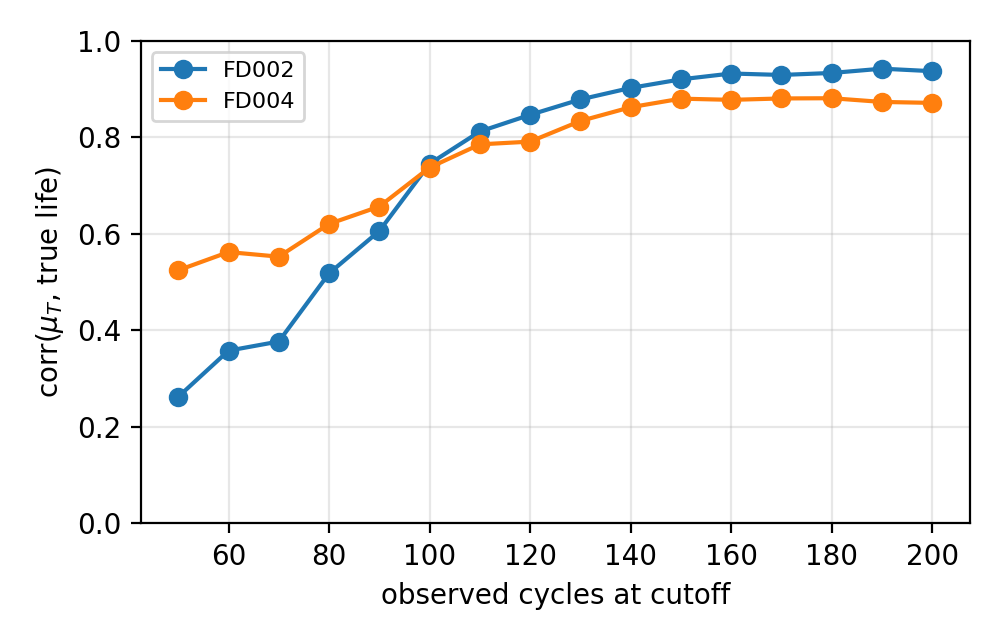
\includegraphics[width=\columnwidth]{fig_observability.png}
\caption{Rank correlation between the lifetime estimate and the true lifetime as a function of the observation cutoff. The scale is essentially unobservable before 100 cycles.}
\label{fig:obs}
\end{figure}

\begin{figure}[t]
\centering
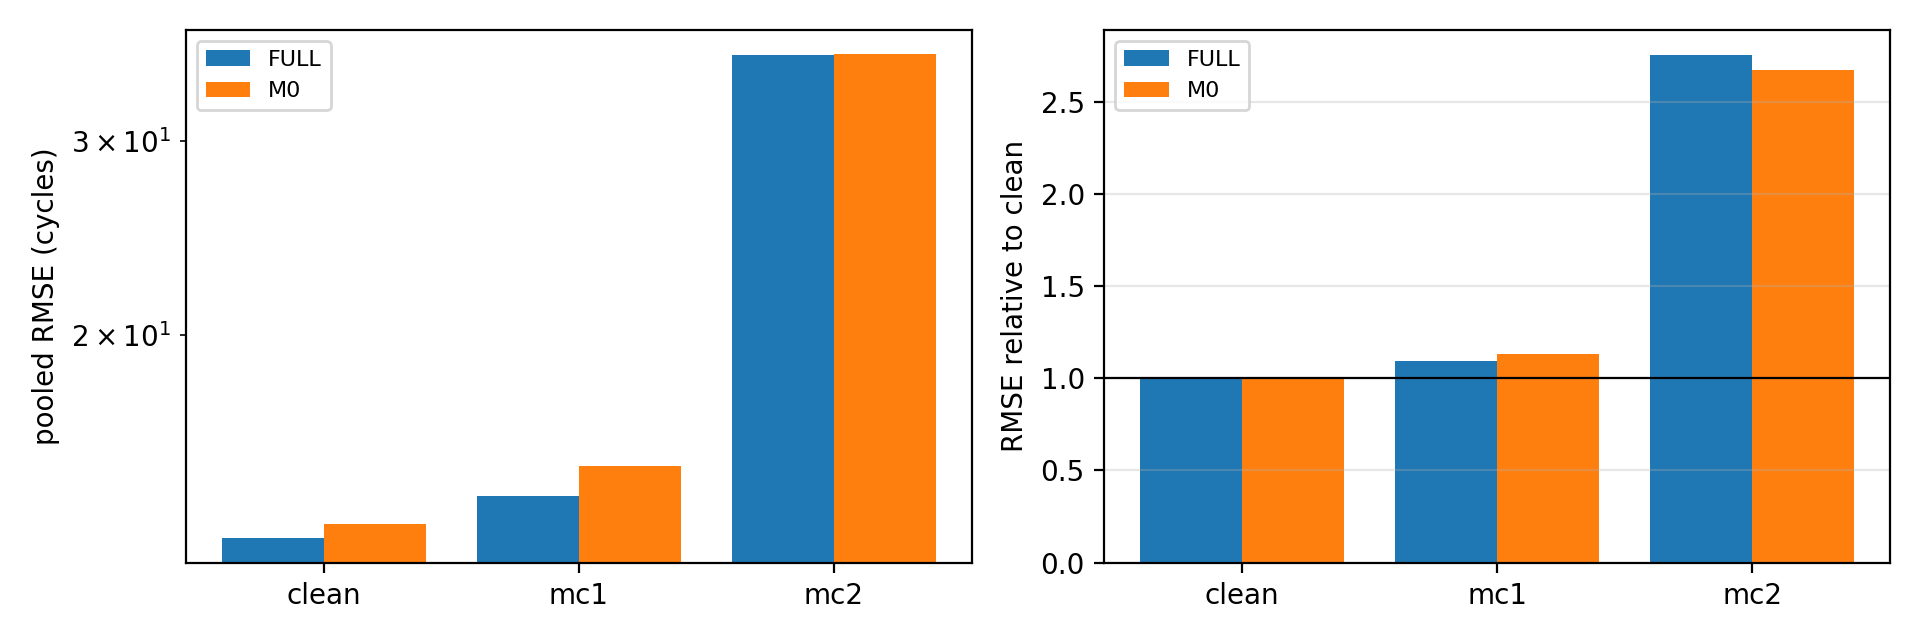
\includegraphics[width=\columnwidth]{fig_measurement_conditions.png}
\caption{Pooled RMSE (left, logarithmic axis) and its ratio to the clean condition (right) under MC1 and MC2.}
\label{fig:mc}
\end{figure}

\begin{figure}[t]
\centering
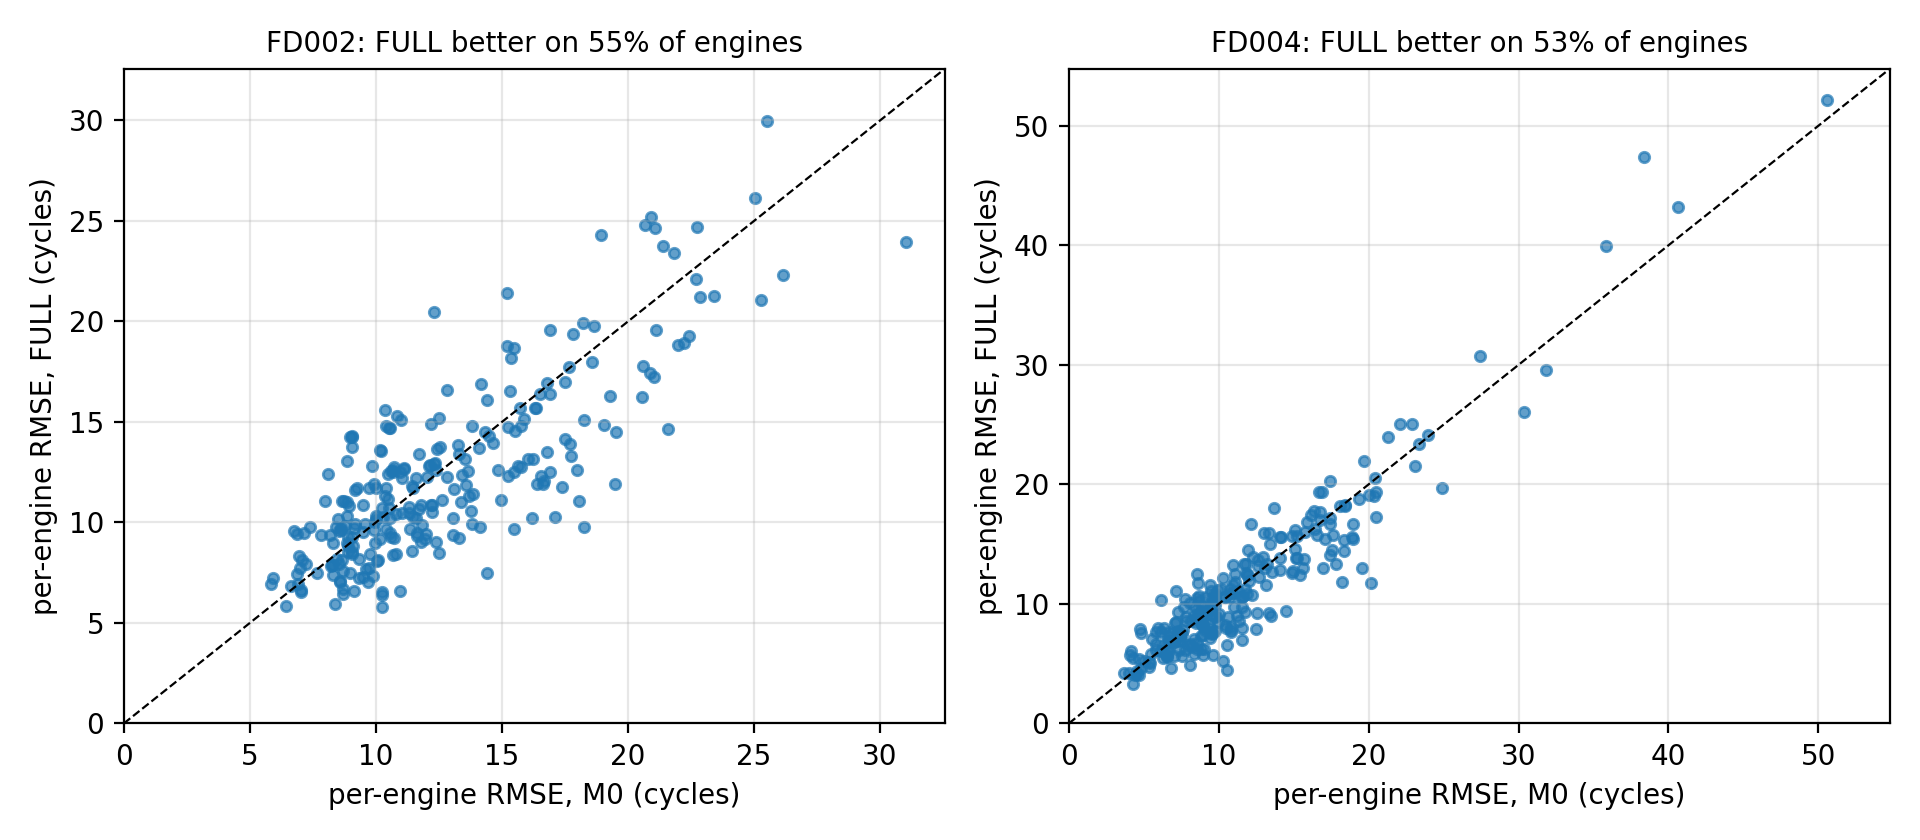
\includegraphics[width=\columnwidth]{fig_per_engine_scatter.png}
\caption{Per-engine RMSE of the plain backbone against the additive-prior arm. The pooled improvement comes from a few large gains outweighing a few large losses.}
\label{fig:eng}
\end{figure}

\begin{figure}[t]
\centering
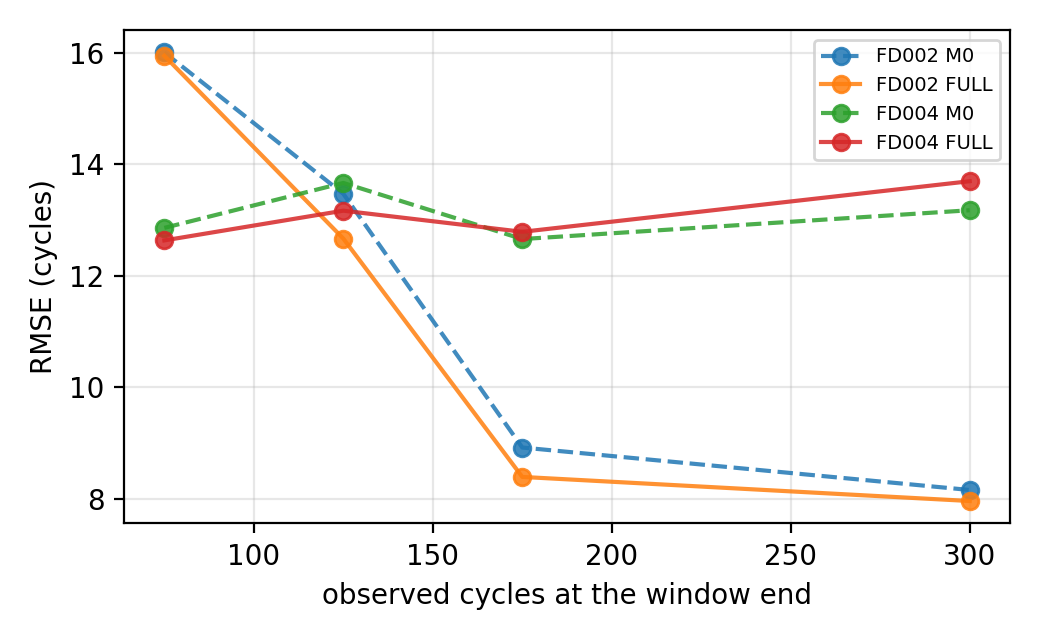
\includegraphics[width=\columnwidth]{fig_error_by_age.png}
\caption{Pooled error against the age of the engine at the prediction time. The gain of the span schedule is concentrated where a long history exists.}
\label{fig:age}
\end{figure}
\subsection{Observation span as a first-order variable}

The protocol fixes the window at 50 cycles. On the windows where a longer history exists, a 100-cycle window lowers the pooled error from 11.03 to 7.50 cycles on FD002 fold 2, and a 150-cycle window reaches 4.97 where it applies. Because a long window is only available once the engine has been observed long enough, we schedule the span to the available history: 50 cycles below 100 observed cycles, 100 cycles above. Both models are trained with the frozen budget.

Across two seeds and five folds, the schedule reduces the pooled RMSE by 7.20 percent on FD002 (MAE 8.312 against 9.158, asymmetric score 3.179 against 3.649) and by 3.89 percent on FD004 (MAE 8.369 against 8.807, asymmetric score 8.682 against 9.943). The stratified interval is 5.53 percent with bounds [0.881, 0.589] cycles, and both subsets are negative for both seeds.

Three controls attribute the gain to the span rather than to specialisation, parameter count or model count. A late-window specialist trained at the same 50-cycle window on the same late windows is worth 3.5 percent. A span control with identical parameter count, which samples 50 positions every second cycle over 100 cycles, is worth 12.8 percent. A three-seed ensemble of the 50-cycle reference, which has the same model count as the schedule, leaves the schedule ahead by 5.8 percent on the fold where both are measured.

\subsection{A pre-registered tail guard}

The schedule is not stable on the asymmetric score. In one seed and one fold a single engine is over-estimated by about 96 cycles; because the score grows exponentially on the over-estimation side, that engine alone contributes 14695 to a fleet mean of 313, against 23 for the reference. The maximum absolute error on that fold is the same for both arms, 124.6 against 124.5; only the sign differs.

We therefore pre-registered a guard before computing any guarded result: when the two models disagree by more than 50 cycles, keep the short-window prediction. The value is about 3.7 times the typical FD004 error, and we report 30, 50 and 75 cycles as a sensitivity check. With the guard the asymmetric score on FD004 falls from 37.76 to 8.68, below the reference value of 9.94, while the RMSE improves from 2.92 to 3.89 percent. The gain is positive for every value in the sensitivity set.

\subsection{What does not work}

The span schedule changes how the measurement is taken. We tested nine model-side interventions with the same recipe, folds and metrics. Table~\ref{tab:neg} reports the single-fold screen against the 42k baseline on the same fold.

\begin{table}[t]
\centering
\caption{Model-side interventions, single-fold screen. Only one cell is clearly positive, and it is on the arm that does not carry the prior.}
\label{tab:neg}
\small
\begin{tabular}{lrrrr}
\toprule
Intervention & FD002 M0 & FD002 FULL & FD004 M0 & FD004 FULL \\
\midrule
Modules (+74k to +677k params) & +7.4\% & +24.9\% & -- & -- \\
A monotonicity loss & +4.3\% & not run & -- & -- \\
B pinball loss & $-$3.9\% & +0.1\% & +5.3\% & +5.8\% \\
C lifetime reparameterisation & +13.8\% & +9.9\% & -- & -- \\
D engine-level mixup & $-$9.1\% & +0.8\% & -- & -- \\
DX mixup, inputs only & +3.5\% & +4.5\% & -- & -- \\
E cross-sensor attention & +6.4\% & -- & -- & -- \\
\bottomrule
\end{tabular}
\end{table}

Three structural conclusions follow. First, the prior arm is saturated: every intervention that helps the no-prior arm returns to zero or reverses on the prior arm, because the zero-initialised injection of the lifetime statistics is itself a strong regulariser. Second, reducing degrees of freedom works on the no-prior arm while adding expressiveness never works, which is consistent with an effective sample size of 208 engines rather than 33k windows. Third, mixup only works when every input channel is mixed consistently: mixing the window and the label but keeping the original prior turns a 9.1 percent gain into a 3.5 percent loss.

\section{Discussion}\label{sec:disc}
The study is simulation-based; the reported RMSE values are estimator performance metrics, not instrument uncertainties, and the intervals are descriptive engine-clustered bootstrap intervals rather than coverage-guaranteed statements. The official test engines have been used by this project before, so those numbers are post-hoc confirmations rather than a blind validation. The FD004, FD001 and FD003 matrices are reported at a single seed; the three-seed requirement is met on FD002. The training script initialises the network before resetting the random seed, so a single run is not bit-reproducible; the multi-seed means are stable (3.37 percent with sd 0.23 percent), so the conclusions rest on them.

\section{Conclusion}\label{sec:concl}
We examined whether the individual lifetime scale that individualisation methods inject into an RUL predictor is observable enough to be used adaptively. On two multi-condition C-MAPSS fleets, under a frozen engine-disjoint protocol, the scale is only partially observable and its observability grows with the observation time; of the three ways it can enter the measurement, only additive injection survives at the full training budget, and none of the observables that the instrument can report predicts when the individual reading should be preferred to a population reference. We conclude that individualisation of RUL measurement in this setting is observability-limited, and we recommend reporting the observability curve, the endpoint and the engine sample alongside any accuracy claim.

\end{document}
